\documentclass[9pt, lualatex]{beamer}

\usepackage{beamerpreamble}

\title{ML techniques in $H^+\to \tau\nu$ mass reconstruction}

\author[Max, Mikael, Camila, Henrik]{
    \underline{Max Isacson}, Mikael Mårtensson,\\ Camila Rangel Smith, Henrik Öhman}

\institute[Uppsala University]{\uulogo}

\date{Statistical Machine Learning, 21 april 2016}

\begin{document}
\frame{\titlepage}

\begin{frame}
    \frametitle{Introduction I}

    \begin{columns}
        \column{.5\textwidth}
    All HEP experiments have to deal with \emph{missing (transverse) energy} (MET, $E_T^\mathrm{miss}$).
    Usually in the form of \emph{neutrinos} escaping the detector without interacting.

        \column{.5\textwidth}
        \begin{figure}
            \centering
            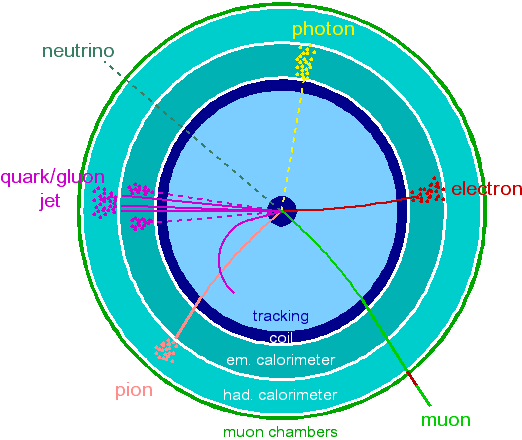
\includegraphics[width=\textwidth]{PID.png}
        \end{figure}

    \end{columns}

    The missing energy can be reconstructed in the transverse plane, by energy conservation:

    \begin{equation}
        E_{x,y}^\text{miss} = -\sum E_{x,y}
    \end{equation}

    However in hadron colliders the longitudinal energy information is lost.

\end{frame}

\begin{frame}
    \frametitle{Introduction II}

    \begin{columns}
        \column{.5\textwidth}
            This is because we are acutally colliding the \emph{partons} inside the hadrons, which carry an unknown
            fraction $x$ of the longitudinal momentum.
        \column{.5\textwidth}
        \begin{figure}
            \centering
            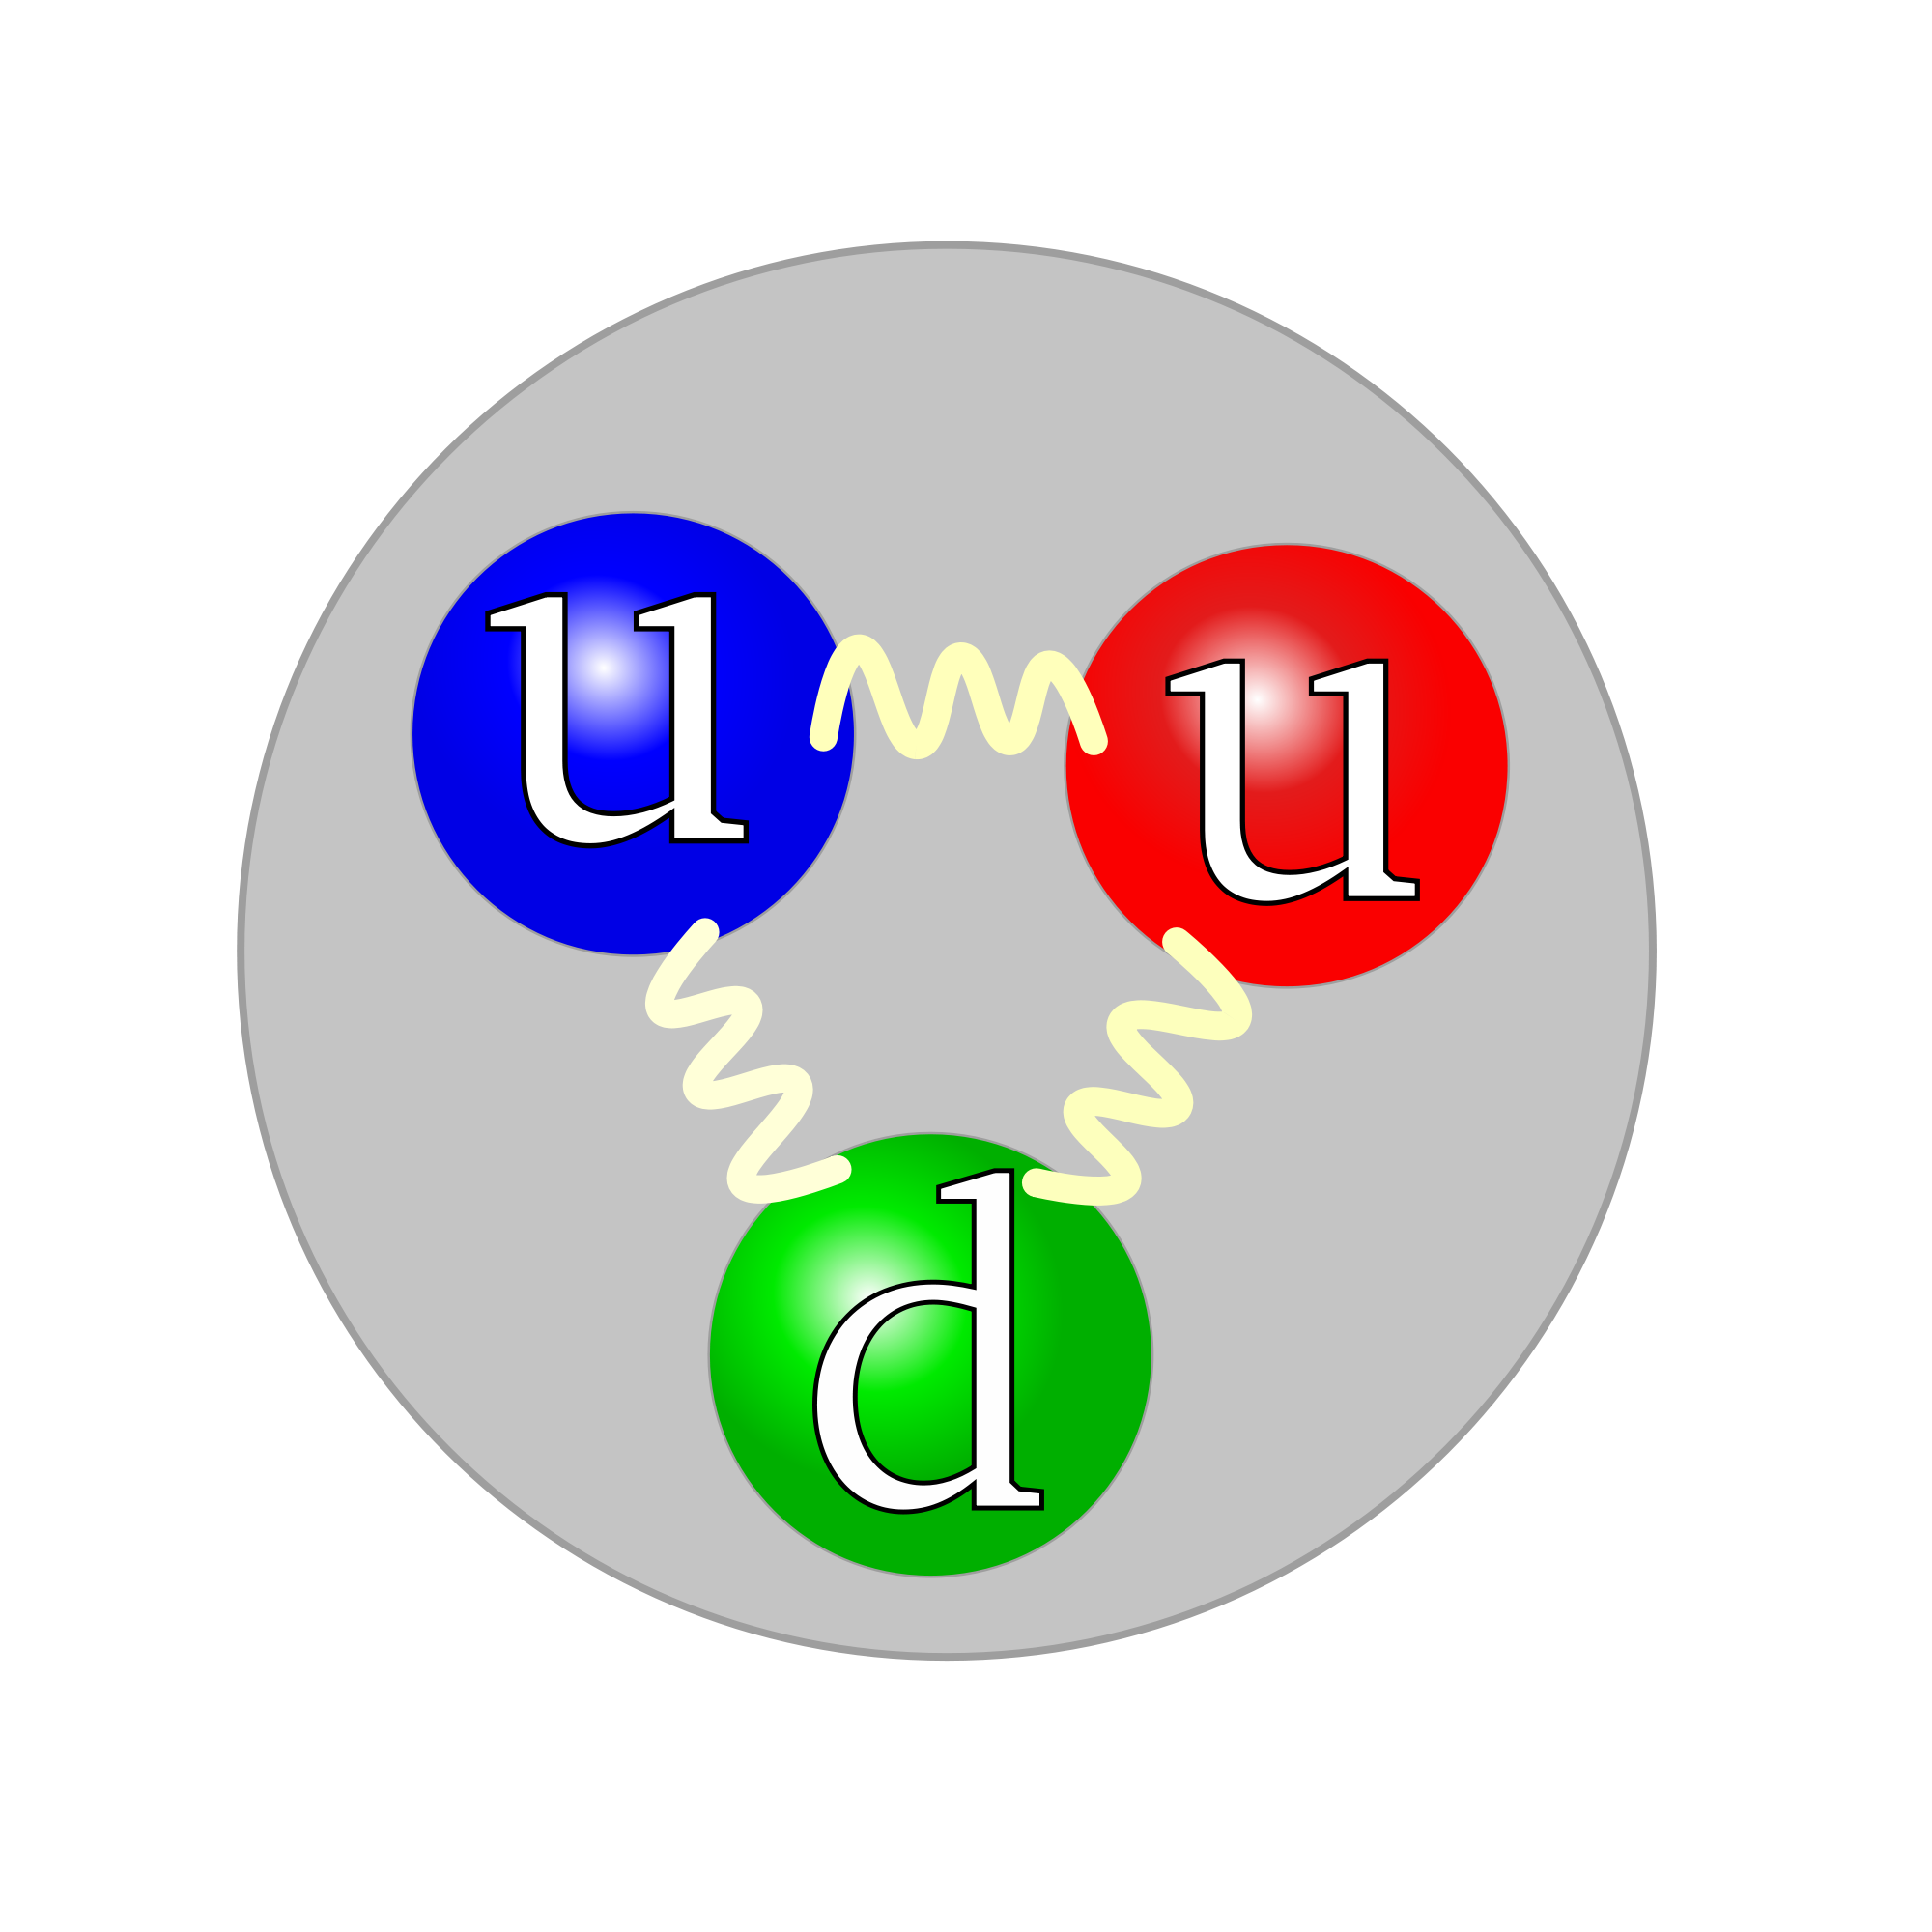
\includegraphics[width=.5\textwidth]{proton.png}
        \end{figure}
    \end{columns}

    \begin{figure}
        \centering
        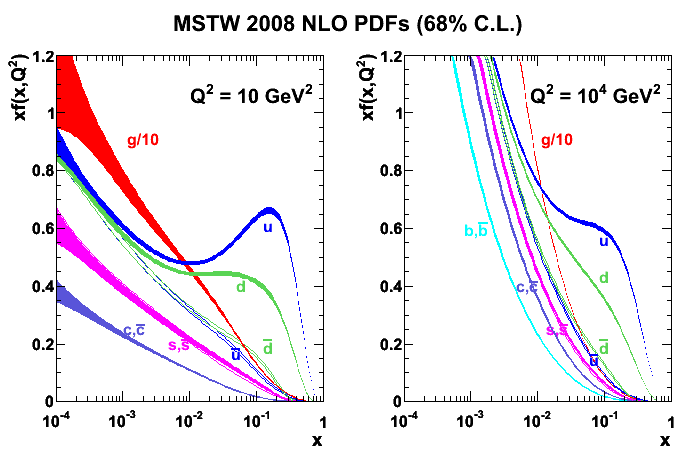
\includegraphics[width=.7\textwidth]{pdf.png}
    \end{figure}

\end{frame}

\begin{frame}
    \frametitle{Definitions}
    \begin{itemize}
        \item Response of $X$ --- The ratio between a reco. quantity $X$ and the true value $X_\text{truth}$, as a function of $X_\text{truth}$.
        \item Resolution of $X$ --- The distribution of $(X_\text{truth} - X)/X_\text{truth}$.
        \item Transverse mass $m_T$ --- The mass in the transverse plane between objects 1 and 2, $m_T = \sqrt{2E_T^1E_T^2(1 - \cos(\phi_1 - \phi_2))}$.
    \end{itemize}
\end{frame}

\begin{frame}
    \frametitle{Signal process}
    \begin{figure}
        \centering
        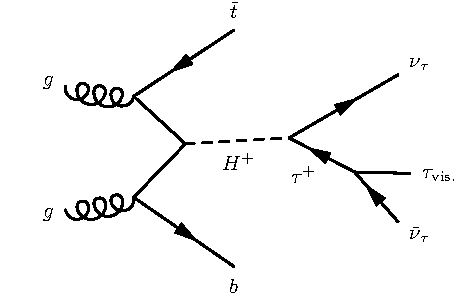
\includegraphics[width=.5\textwidth]{heavyHplustaunu4fs.pdf}
    \end{figure}

    \begin{itemize}
        \item Most of the missing energy will be carried by $\nu_H$ --- The neutrino from the Higgs decay.
        \item The features used are the various kinematics of the visible part of this process.
        \item We consider 3 masses for the $H^+$: 200, 300, and 400 GeV
    \end{itemize}

\end{frame}

\begin{frame}
    \frametitle{Predictors}
    \begin{columns}
        \column{.5\textwidth}
        \centering
        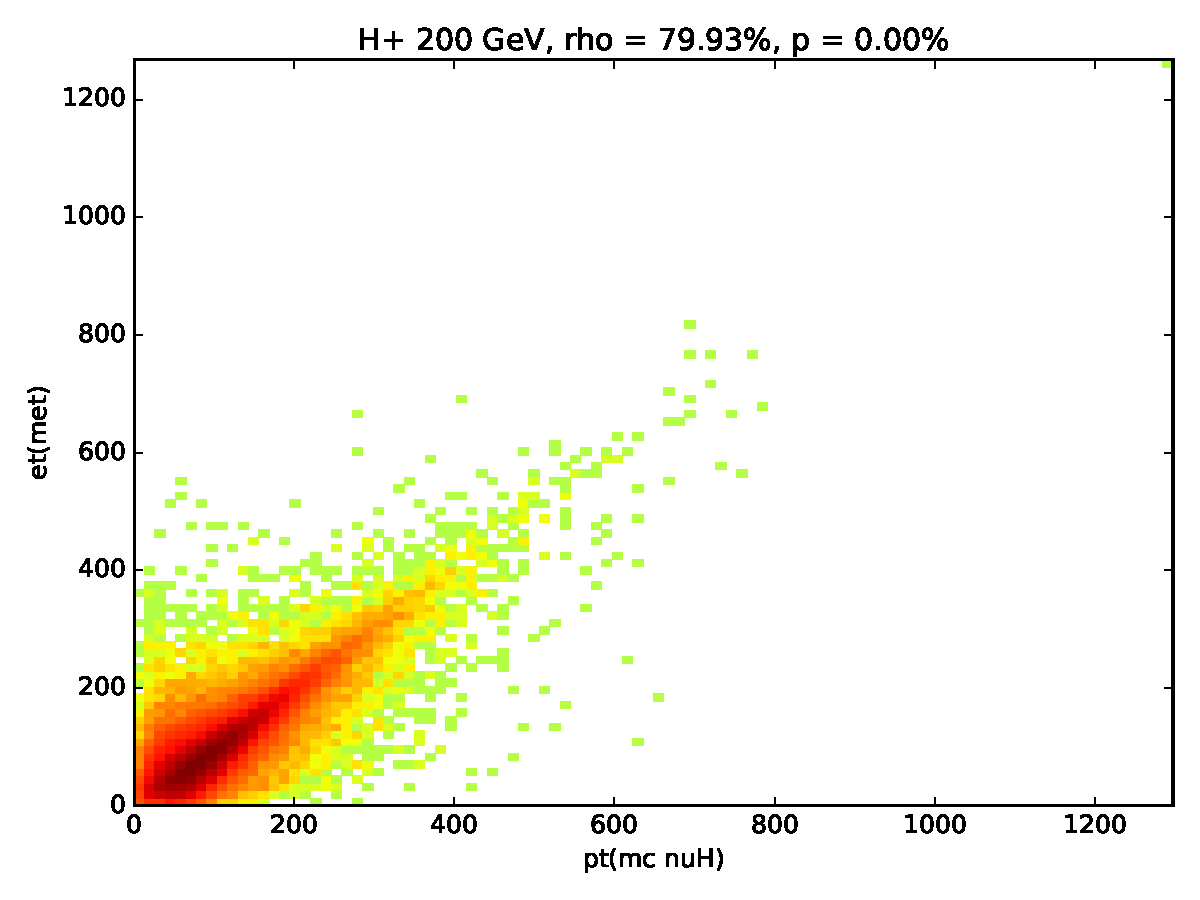
\includegraphics[width=\textwidth]{correlations/hp200_et_met.pdf}\\
        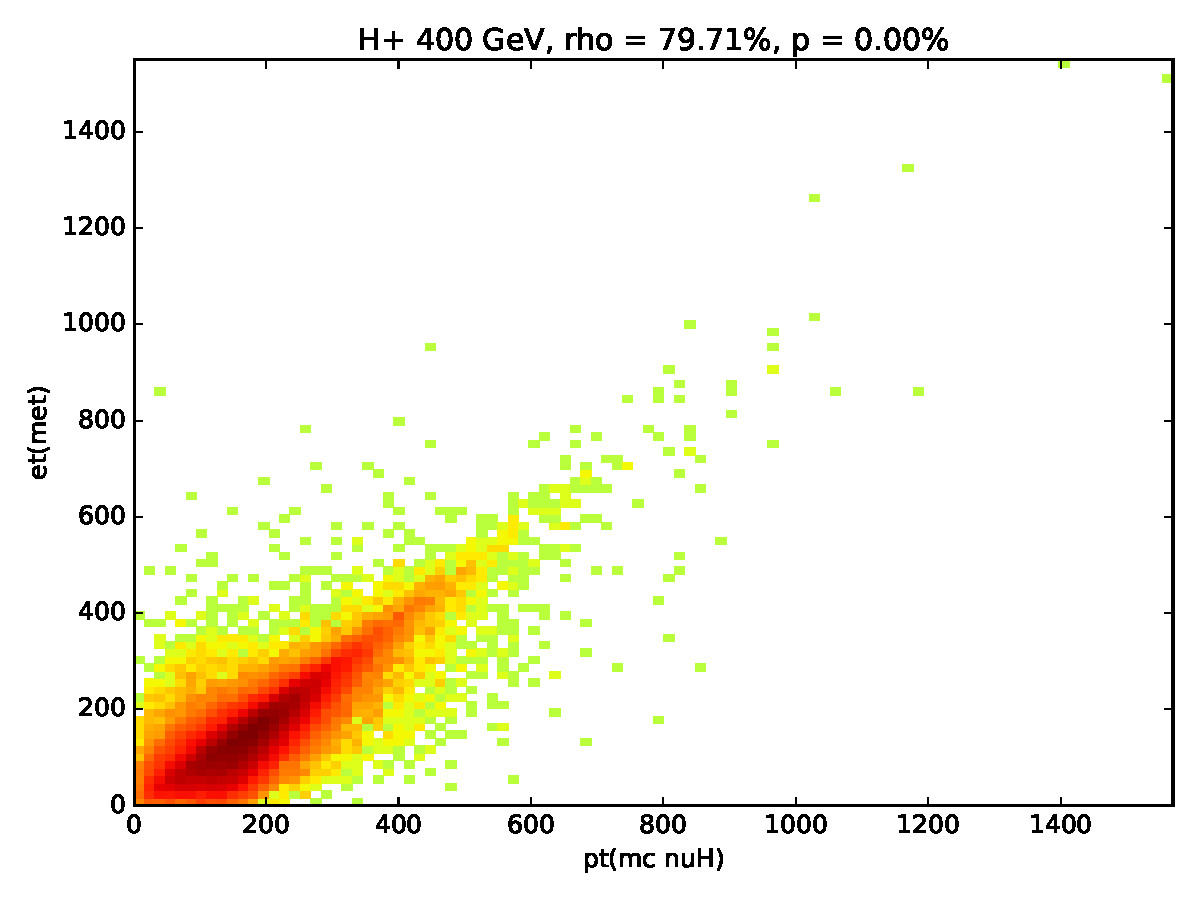
\includegraphics[width=\textwidth]{correlations/hp400_et_met.pdf}
        \column{.5\textwidth}
        \centering
        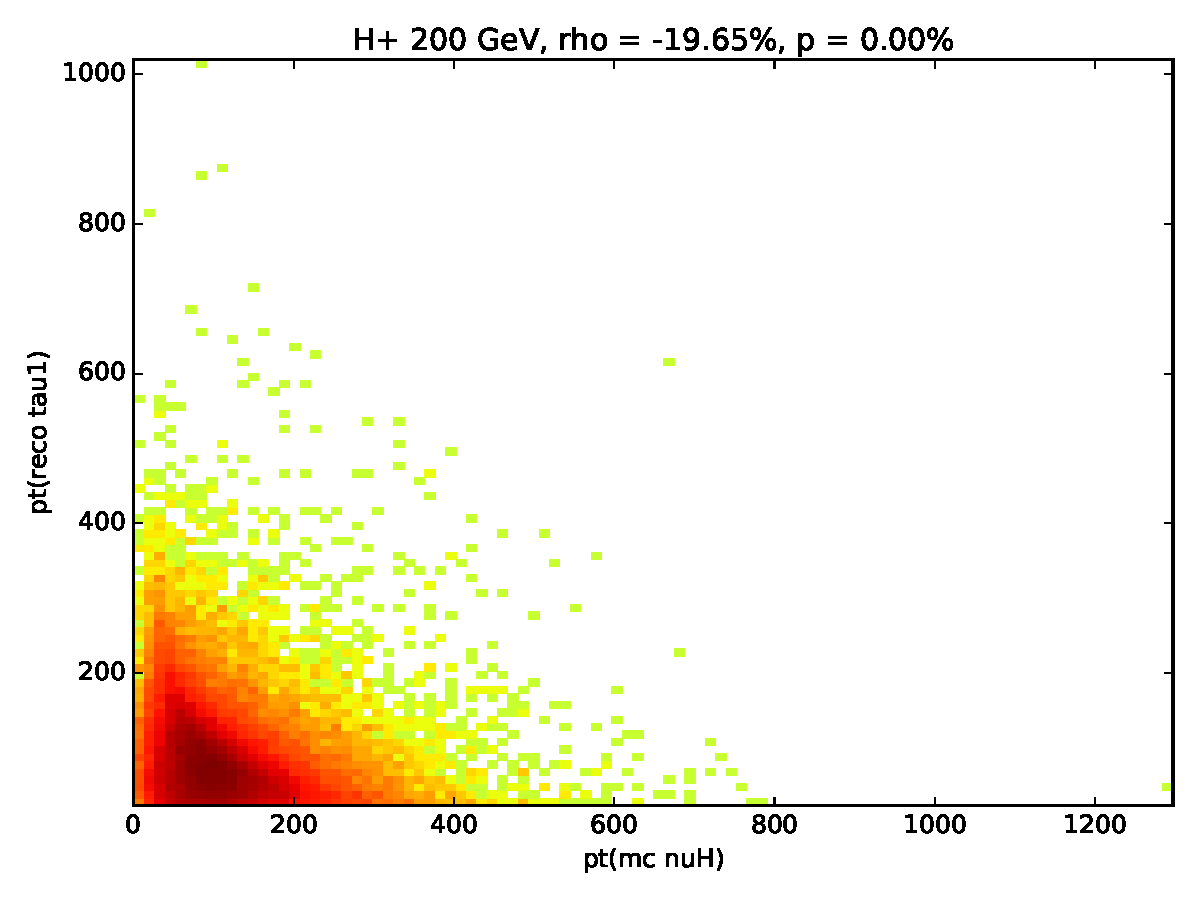
\includegraphics[width=\textwidth]{correlations/hp200_pt_reco_tau1.pdf}\\
        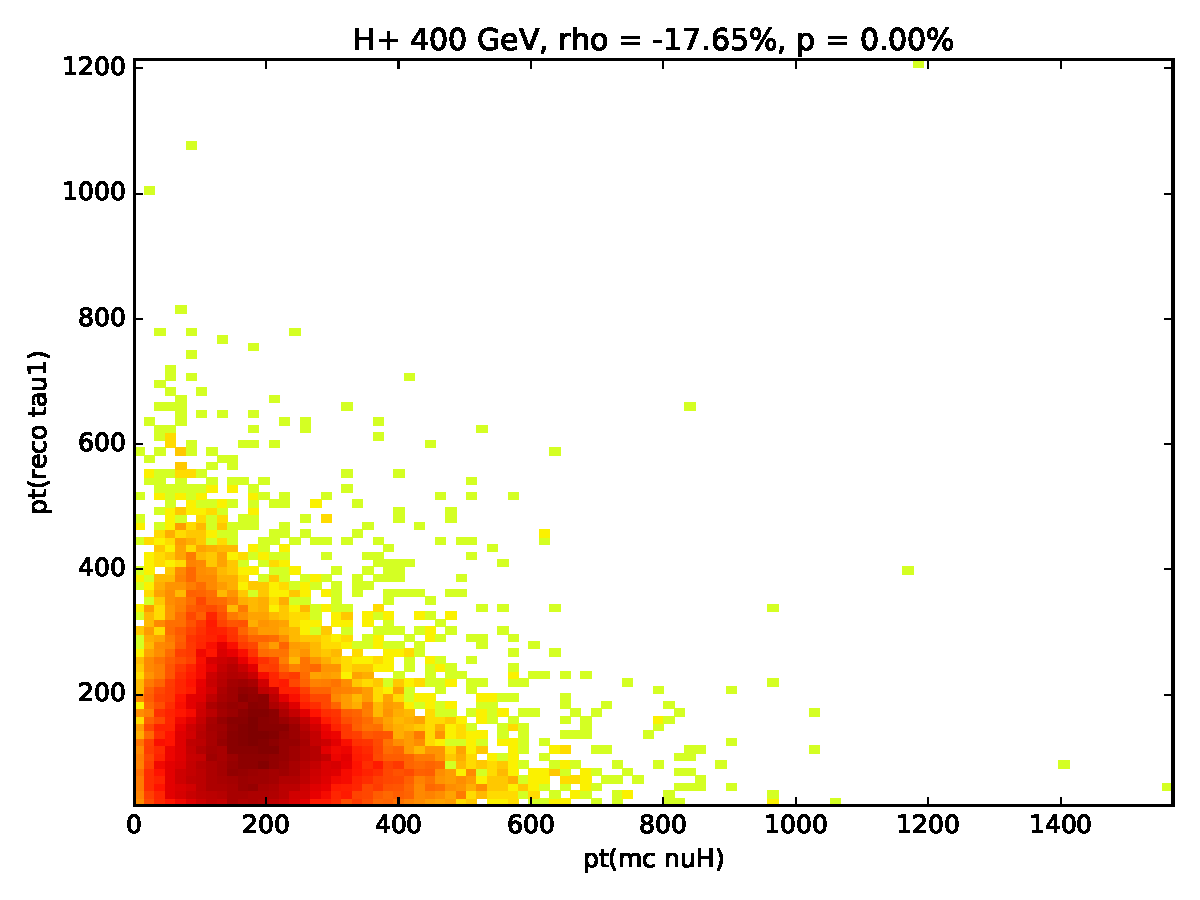
\includegraphics[width=\textwidth]{correlations/hp400_pt_reco_tau1.pdf}
    \end{columns}

\end{frame}

\begin{frame}
    \frametitle{Regressors}
    \begin{itemize}
    \item Gaussian process
    \item Neural network
    \item Bayesian ridge regression
    \item Support vector regression
    \end{itemize}
    \vfill
    \begin{itemize}
        \item The target for the training is always the $p_T$ of $\nu_H$.
        \item We consider 4 measures of quality, the distribution of the predicted $p_T$, the response, the resolution,
            and the reconstructed $m_T$ using the predicted $p_T$.
        \item These are compared to the standard MET.
    \end{itemize}
\end{frame}

\begin{frame}
    \frametitle{Reconstruction of $p_{T}(\nu_H)$}

    \begin{figure}
        \centering
        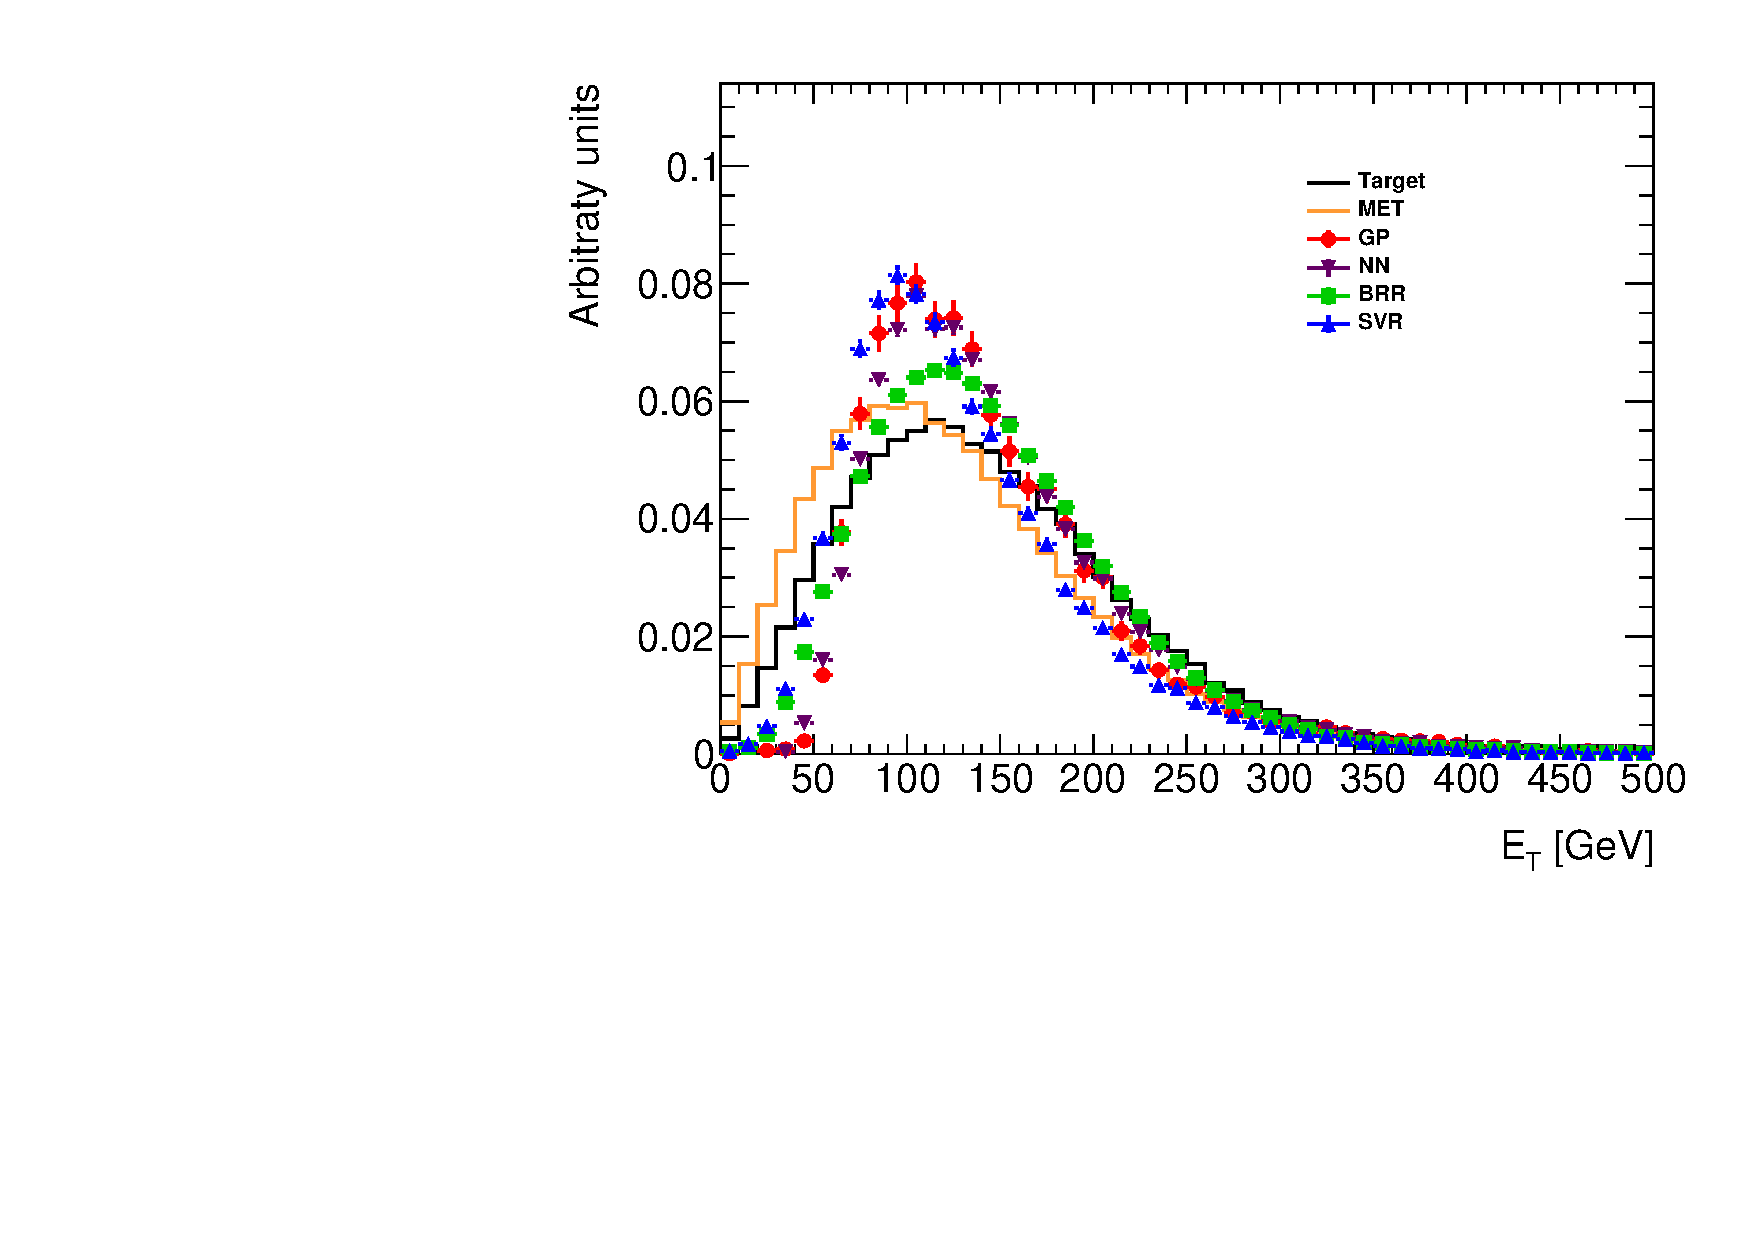
\includegraphics[width=.7\textwidth]{plots/pt.pdf}
    \end{figure}
\end{frame}

\begin{frame}
    \frametitle{$p_{T}$ response}

    \begin{figure}
        \centering
        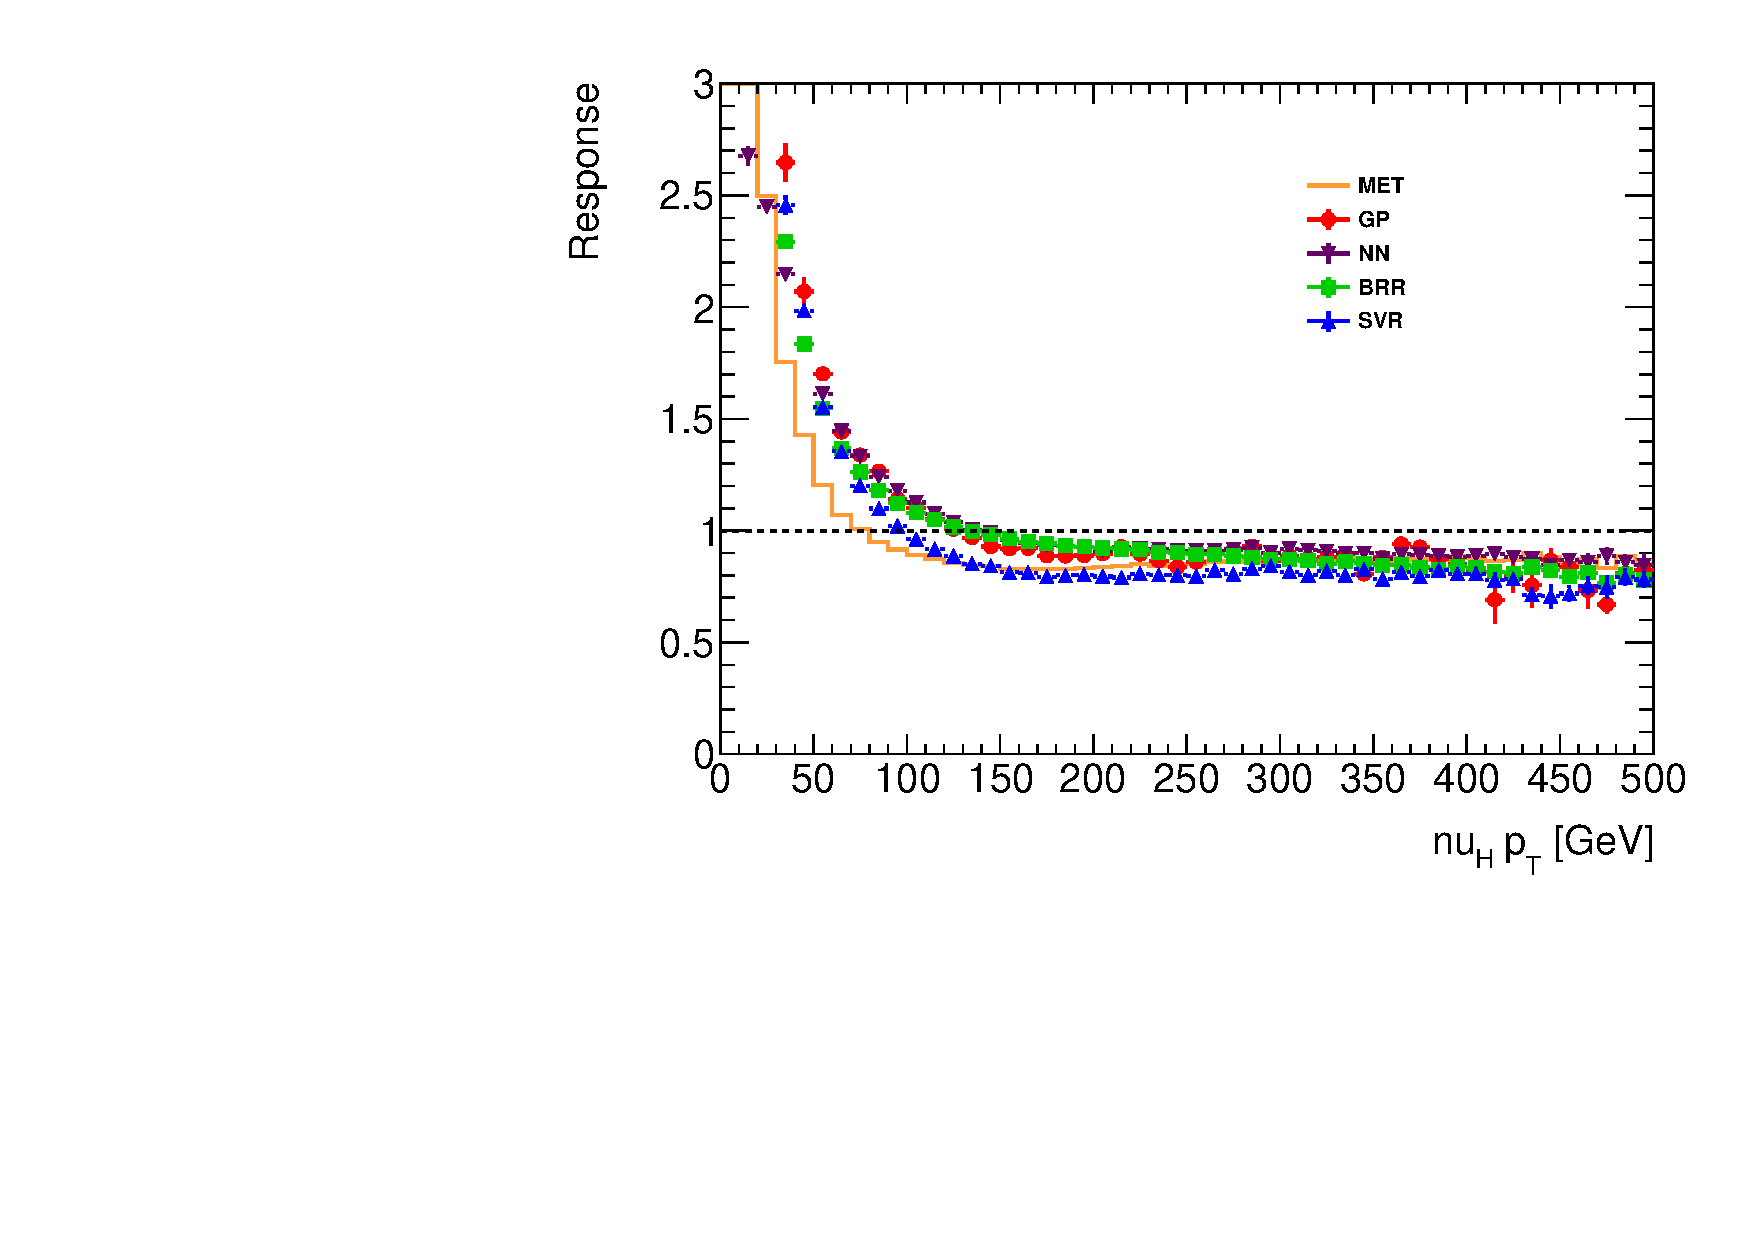
\includegraphics[width=.7\textwidth]{plots/profile.pdf}
    \end{figure}
\end{frame}

\begin{frame}
    \frametitle{$p_{T}$ resolution}

    \begin{figure}
        \centering
        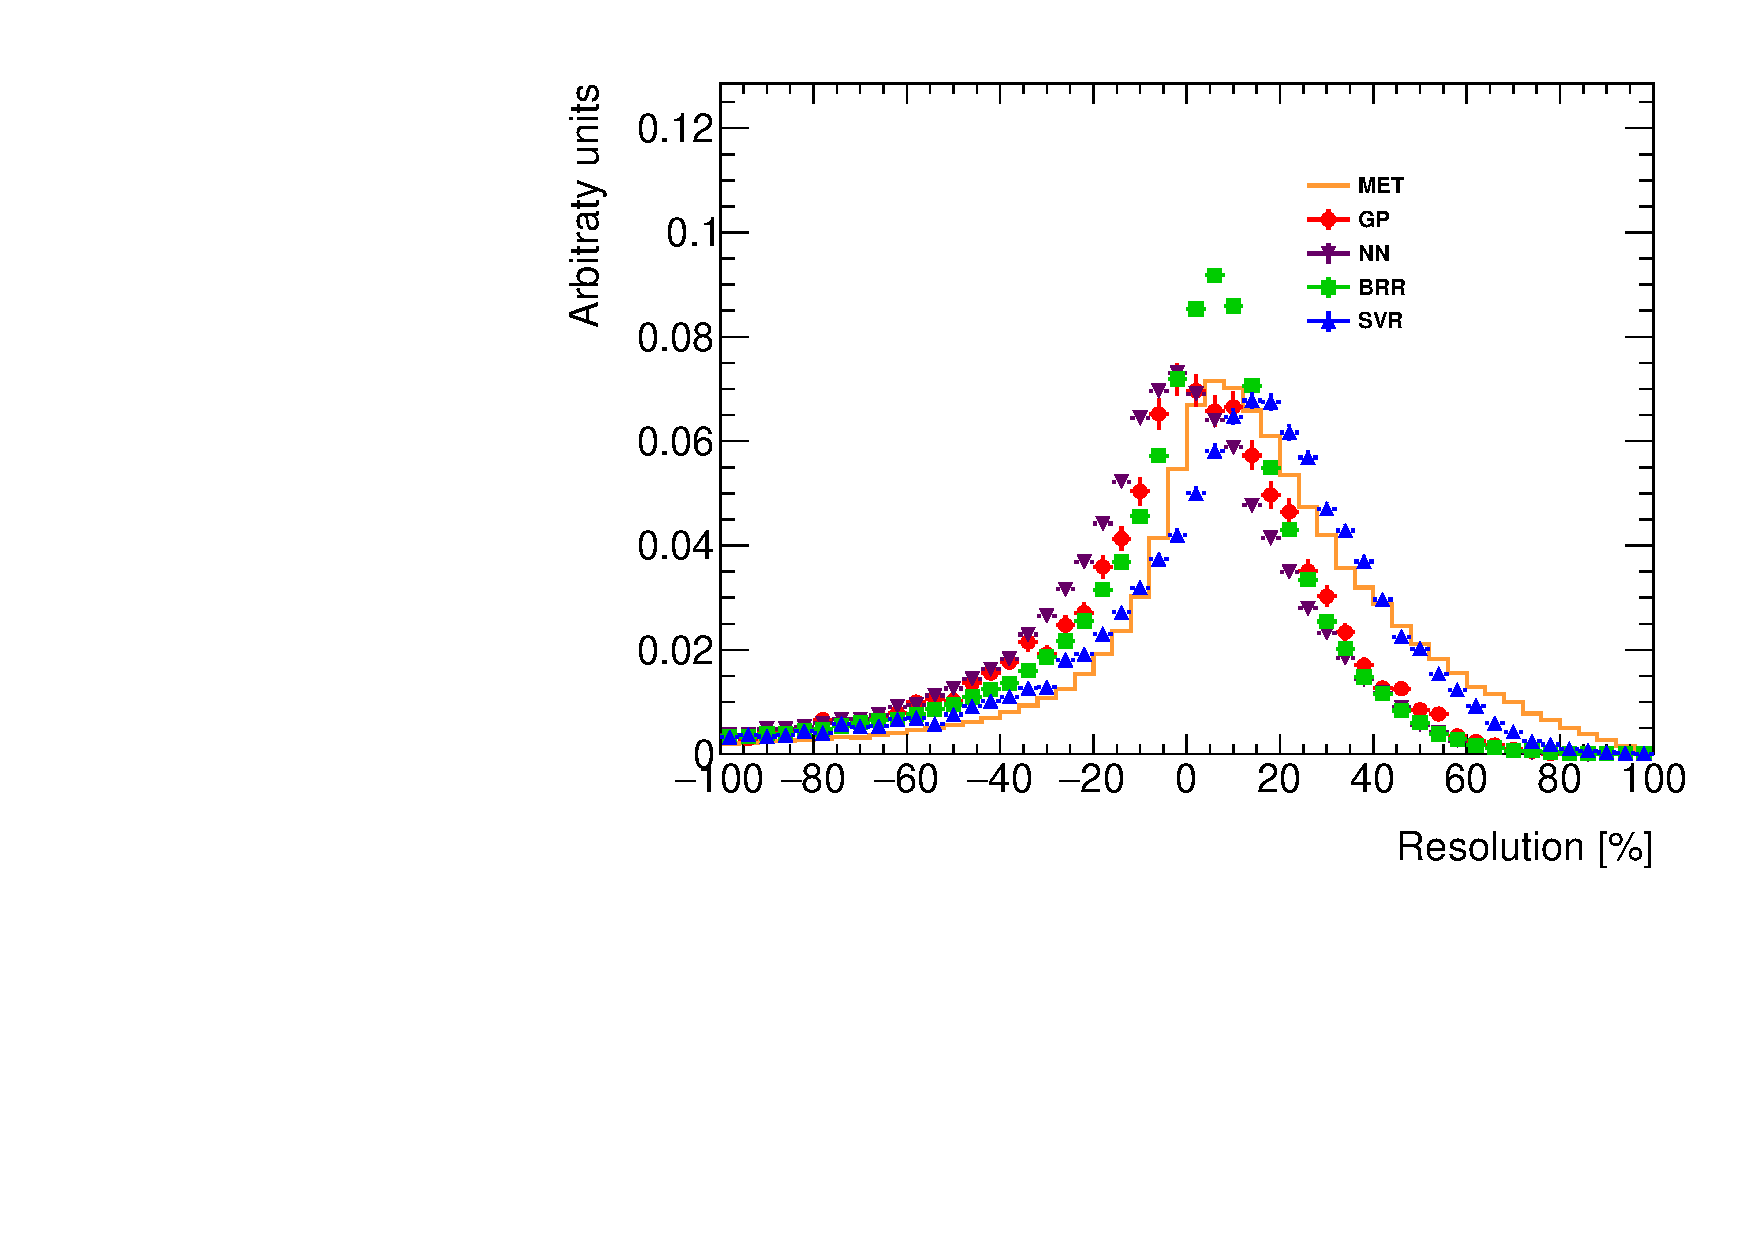
\includegraphics[width=.7\textwidth]{plots/resolution.pdf}
    \end{figure}
\end{frame}

\begin{frame}
    \frametitle{Reconstruction of $m_T$}

    \begin{figure}
        \centering
        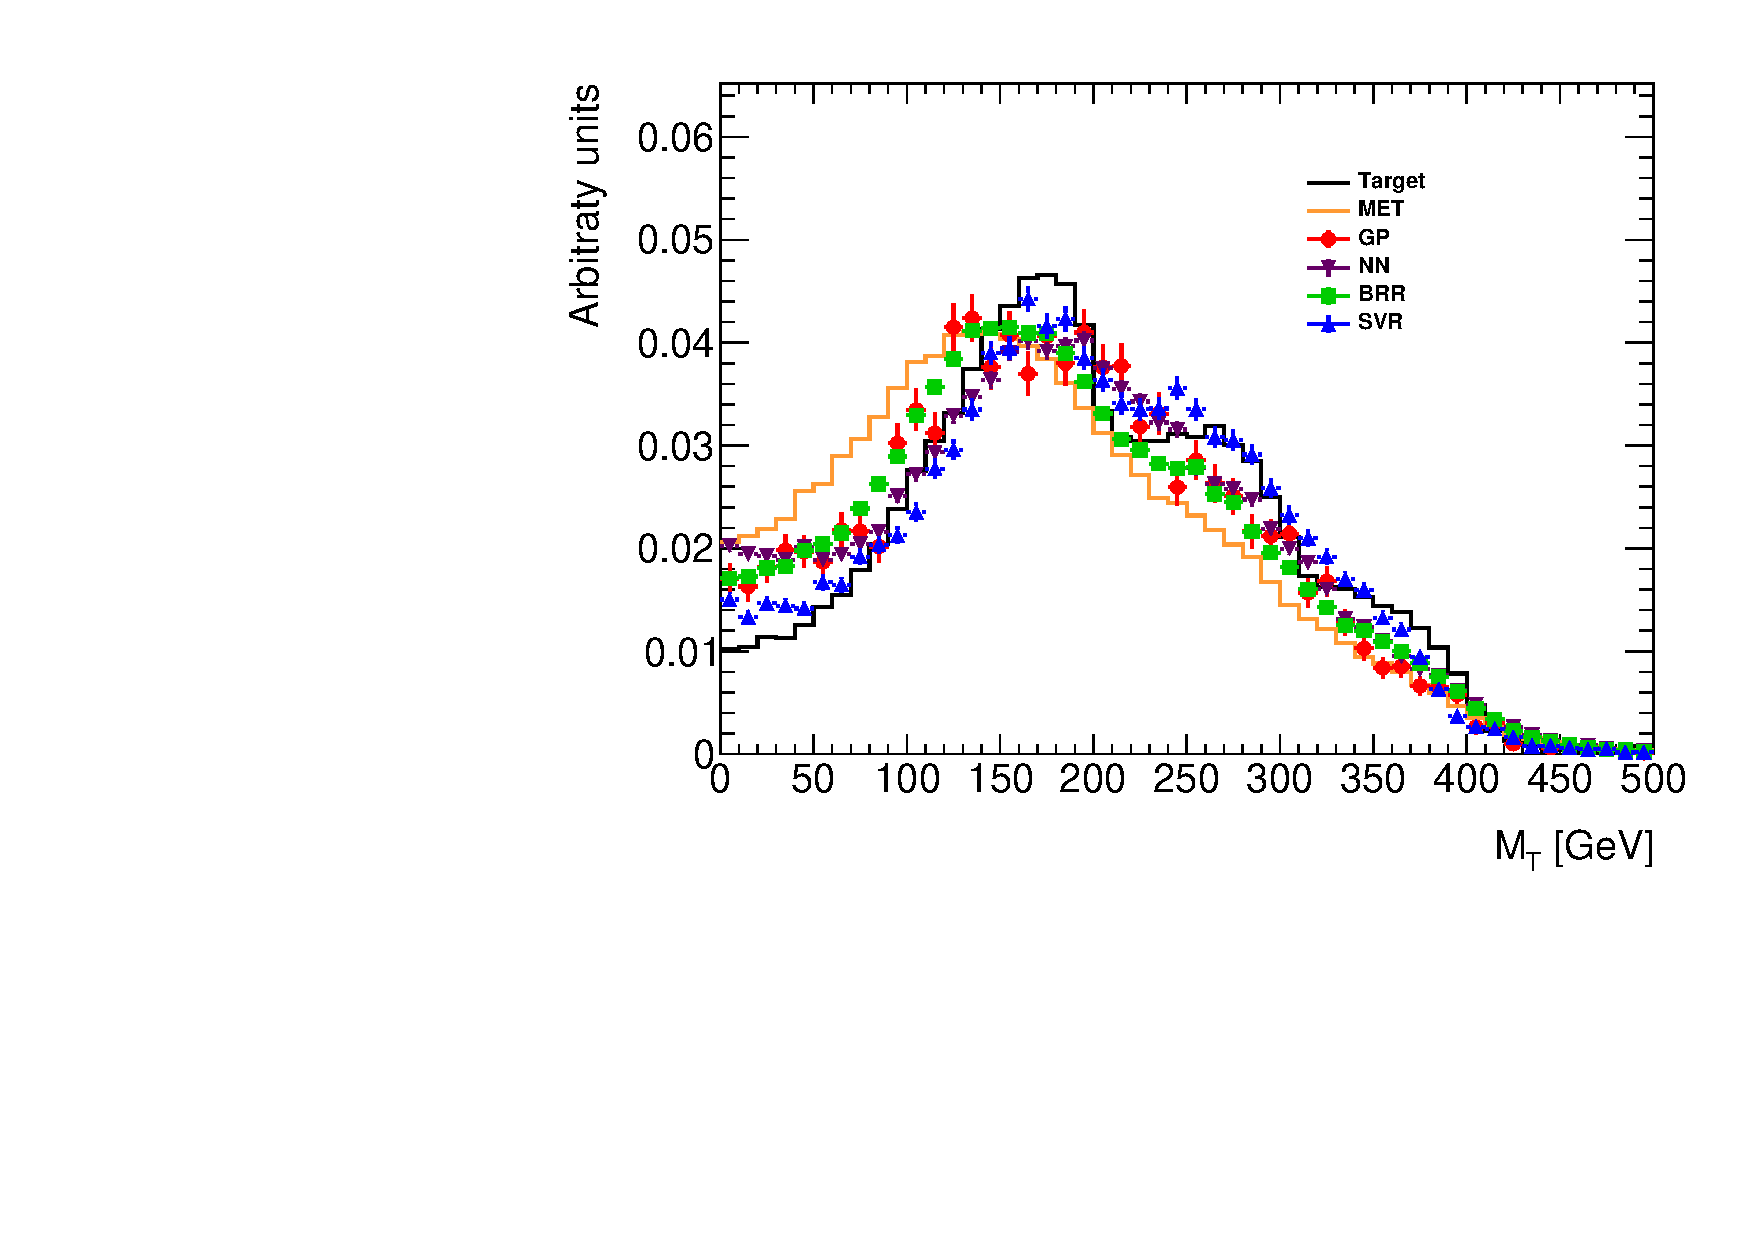
\includegraphics[width=.7\textwidth]{plots/mt.pdf}
    \end{figure}
\end{frame}

\begin{frame}
    \frametitle{Conclusions and plans}

    Conclusions
    \begin{itemize}
        \item The neural network and bayesian ridge regression are the best performers.
        \item NN has the smallest bias, but larger variance than the BRR.
        \item However, all methods fails to reconstruct the spectrum at low $p_T$.
        \item More detailed studies has to be performed to draw more accurate conclusions.
    \end{itemize}

    \vfill

    Plans
    \begin{itemize}
        \item We plan to continue this in the future -- Will be of interest to HBSM searches at ATLAS and other hadron experiments.
        \item The performance will probably be better when training against the full 4-vector of $\nu_H$.
        \item More complicated variables could also be included in the training.
    \end{itemize}
\end{frame}

\end{document}

